% file: qtree-branch-position.tex
% see: [How to specify branch positions in tikz-qtree @ TeX?](https://tex.stackexchange.com/q/405440/23098)

\documentclass{standalone}

\usepackage{tikz}
\usepackage{tikz-qtree}
\usetikzlibrary{positioning}

\begin{document}
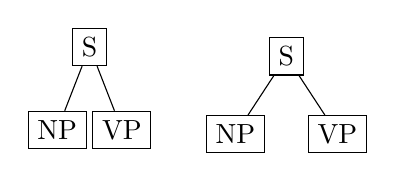
\begin{tikzpicture}[every node/.style = {draw, rectangle},
  edge from parent/.style= {
  	draw, edge from parent path={(\tikzparentnode) -- (\tikzchildnode)}},]
  % using tikz-qtree
  \Tree [.S [.NP ]
  	    [.VP ]
	]

  % desired: both branches do not come from ''s.south''
  \begin{scope}[xshift = 2.5cm]
    \node (s) {S};
    \node (np) [below left = 0.50cm and 0.05cm of s] {NP};
    \node (vp) [below right = 0.50cm and 0.05cm of s] {VP};
    \draw (s) to (np);
    \draw (s) to (vp);
  \end{scope}
\end{tikzpicture}
\end{document}